\section{Goods and Services}
The world of Athas has a very specific feel to it; many things that are taken for granted in other campaign worlds, like the availability of metal and water, are very different on this heat-wracked planet. To maintain this feel, the equipment available to characters should reflect these differences.

\begin{figure*}[t!]
\centering
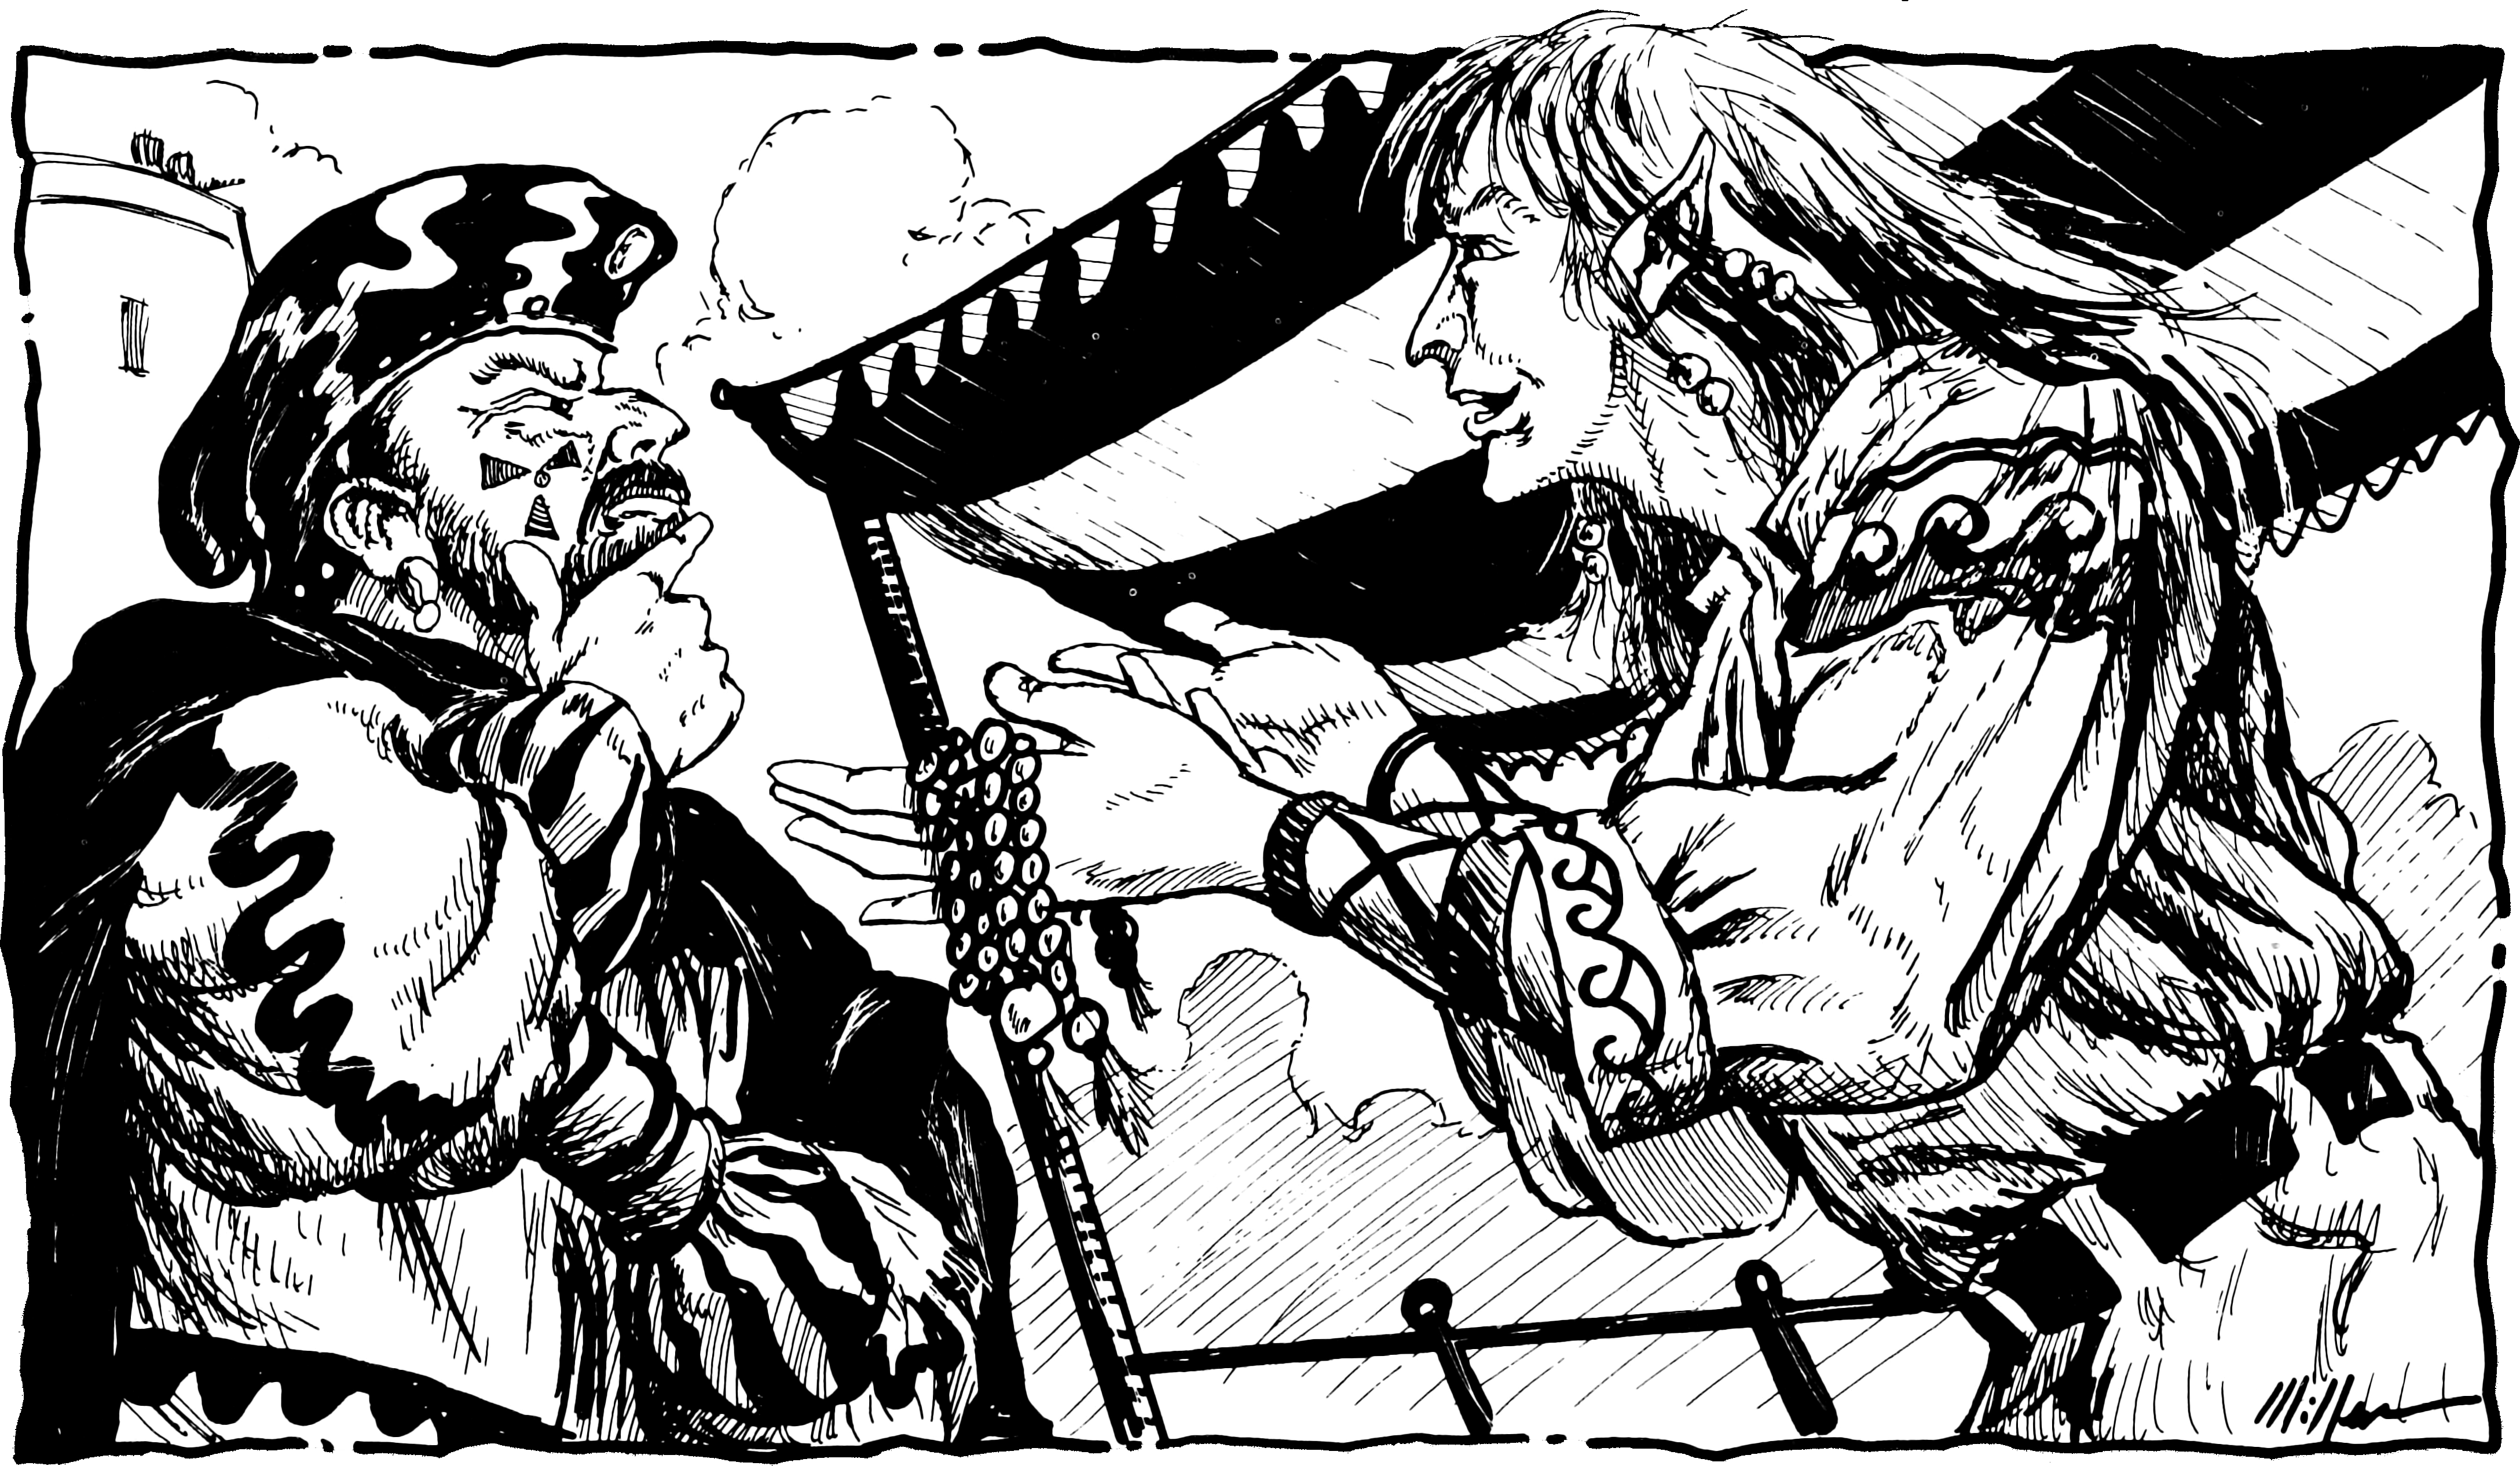
\includegraphics[width=\textwidth]{images/merchant-1.png}
\par\textit{\small\textcopyright Wizards of the Coast, 2020.}
\end{figure*}

\subsection{Adventuring Gear}

\Table{Adventuring Gear}{l RRRR}{
&& \multicolumn{3}{c}{\tableheader Weight}\\
\cmidrule[0.5pt]{3-5}
\tableheader Goods & \tableheader Cost & \tableheader M & \tableheader S & \tableheader L\\
Backpack (empty) & 2 cp & 1 kg & 0.25 kg & 4 kg\\
Barrel (empty) & 2 cp & 15 kg & &\\
Basket (empty) & 4 bits & 0.5 kg & &\\
Bedroll & 1 bits & 2.5 kg & 2.5 kg & 2.5 kg\\
Bell & 1 cp & & &\\
Blanket, winter & 5 bits & 1.5 kg & 0.37 kg & 6 kg\\
Block and tackle & 5 cp & 2.5 kg & &\\
Bottle, wine, glass & 2 cp & & &\\
Bucket (empty) & 5 bits & 1 kg & &\\
Caltrops & 1 cp & 1 kg & &\\
Candle & 1 bd & & &\\
Canvas (sq. m.) & 1 bits & 0.5 kg & &\\
Case, map or scroll & 1 cp & 0.25 kg & &\\
Chain (3 m.) & 30 cp & 1 kg & &\\
Chalk, 1 piece & 1 bd & & &\\
Chest (empty) & 2 cp & 12.5 kg & &\\
Crowbar & 2 cp & 2.5 kg & &\\
Firewood (per day) & 1 bd & 10 kg & &\\
Fishhook & 1 bits & & &\\
Fishing net, 2 sq. m. & 4 cp & 2.5 kg & &\\
Flask (empty) & 3 bd & 0.75 kg & &\\
Flint and steel & 1 cp & & &\\
Grappling hook & 1 cp & 2 kg & &\\
Hammer & 5 bits & 1 kg & &\\
Ink (30 ml vial) & 8 cp & & &\\
Inkpen & 1 bits & & &\\
Jug, clay & 3 bd & 9 lb. & &\\
Ladder, 3-meter & 5 bd & 10 kg & &\\
Lamp, common & 1 bits & 0.5 kg & &\\
Lantern, bullseye & 12 cp & 1.5 kg & &\\
Lantern, hooded & 7 cp & 1 kg & &\\
Lock (very simple) & 20 cp & 0.5 kg & &\\
Lock (average) & 40 cp & 0.5 kg & &\\
Lock (good) & 80 cp & 0.5 kg & &\\
Lock (amazing) & 150 cp & 0.5 kg & &\\
Manacles & 15 cp & 1 kg & &\\
Manacles, masterwork & 50 cp & 1 kg & &\\
Mirror, small steel & 10 cp & 0.25 kg & &\\
Mug/Tankard, clay & 2 bd & 0.5 kg & &\\
Oil (500 ml flask) & 1 bits & 0.5 kg & &\\
Paper (sheet) & 4 bits & & &\\
Parchment (sheet) & 2 bits & & &\\
Pick, miner's & 3 cp & 5 kg & &\\
Pitcher, clay & 2 bd & 2.5 kg & &\\
Piton & 1 bits & 0.25 kg & &\\
Pole, 3-meter & 2 bits & 4 kg & &\\
Pot, iron & 5 bits & 5 kg & &\\
Pouch, belt (empty) & 1 cp & 0.25 kg & 0.06 kg & 1 kg\\
Ram, portable & 10 cp & 10 kg & &\\
Rations, trail (per day) & 5 bits & 0.5 kg & 0.12 kg & 2 kg\\
Rope, giant hair (15 m.) & 50 cp & 5 kg & &\\
Rope, hempen (15 m.) & 1 cp & 5 kg & &\\
Rope, silk (15 m.) & 10 cp & 2.5 kg & &\\
Sack (empty) & 1 bits & 0.25 kg & 0.06 kg & 1 kg\\
Sealing wax & 1 cp & 0.5 kg & &\\
Sewing needle & 5 bits & & &\\
Signal whistle & 8 bits & & &\\
Signet ring & 5 cp & & &\\
Sledge & 1 cp & 5 kg & &\\
Soap (per 0.5 kg) & 5 bits & 0.5 kg & &\\
Spade or shovel & 2 cp & 4 kg & &\\
Spyglass & 1,000 cp & 0.5 kg & &\\
Tent & 10 cp & 10 kg & 2.5 kg & 40 kg\\
Torch & 1 bd & 0.5 kg & &\\
Vial, ink or potion & 1 cp & 0.05 kg & &\\
Waterskin & 1 cp & 2 kg & 0.5 kg & 8 kg\\
Whetstone & 2 bd & 0.5 kg & &\\
}


Some items weight differently for Small or Large characters, these items weigh one-quarter of the Medium-sized when made for Small characters and weigh four times as much the normal weight when made for Large characters. Containers for Small characters also carry one-quarter the normal amount, while containers for Large characters carry four times as much the normal amount.

A few of the pieces of adventuring gear are described below, along with any special benefits they confer on the user (``you'').


\textbf{Caltrops:} A caltrop is a four-pronged iron spike crafted so that one prong faces up no matter how the caltrop comes to rest. You scatter caltrops on the ground in the hope that your enemies step on them or are at least forced to slow down to avoid them. One 1-kilogram bag of caltrops covers an area 1.5 meter square.

Each time a creature moves into an area covered by caltrops (or spends a round fighting while standing in such an area), it might step on one. The caltrops make an attack roll (base attack bonus +0) against the creature. For this attack, the creature's shield, armor, and deflection bonuses do not count. If the creature is wearing shoes or other footwear, it gets a +2 armor bonus to AC. If the caltrops succeed on the attack, the creature has stepped on one. The caltrop deals 1 point of damage, and the creature's speed is reduced by one-half because its foot is wounded. This movement penalty lasts for 24 hours, or until the creature is successfully treated with a DC 15 \skill{Heal} check, or until it receives at least 1 point of magical curing. A charging or running creature must immediately stop if it steps on a caltrop. Any creature moving at half speed or slower can pick its way through a bed of caltrops with no trouble.

Caltrops may not be effective against unusual opponents.

\textbf{Candle:} A candle dimly illuminates a 1.5-meter radius and burns for 1 hour.

\textbf{Chain:} Chain has hardness 10 and 5 hit points. It can be burst with a DC 26 Strength check.

\textbf{Crowbar:} A crowbar grants a +2 circumstance bonus on Strength checks made for such purposes. If used in combat, treat a crowbar as a one-handed improvised weapon that deals bludgeoning damage equal to that of a club of its size.

\textbf{Flint and Steel:} Lighting a torch with flint and steel is a full-round action, and lighting any other fire with them takes at least that long.

\textbf{Grappling Hook:} Throwing a grappling hook successfully requires a \skill{Use Rope} check (DC 10, +2 per 3 meters of distance thrown).

\textbf{Hammer:} If a hammer is used in combat, treat it as a one-handed improvised weapon that deals bludgeoning damage equal to that of a spiked gauntlet of its size.

\textbf{Ink:} This is black ink. You can buy ink in other colors, but it costs twice as much.

\textbf{Jug, Clay:} This basic ceramic jug is fitted with a stopper and holds 4 liters of liquid.

\textbf{Lamp, Common:} A lamp clearly illuminates a 4.5-meter radius, provides shadowy illumination out to a 9-meter radius, and burns for 6 hours on 500 ml of oil. You can carry a lamp in one hand.

\textbf{Lantern, Bullseye:} A bullseye lantern provides clear illumination in a 18-meter cone and shadowy illumination in a 36-meter cone. It burns for 6 hours on 500 ml of oil. You can carry a bullseye lantern in one hand.

\textbf{Lantern, Hooded:} A hooded lantern clearly illuminates a 9-meter radius and provides shadowy illumination in a 18-meter radius. It burns for 6 hours on 500 ml of oil. You can carry a hooded lantern in one hand.

\textbf{Lock:} The DC to open a lock with the \skill{Open Lock} skill depends on the lock's quality: simple (DC 20), average (DC 25), good (DC 30), or superior (DC 40).

\textbf{Manacles and Manacles, Masterwork:} Manacles can bind a Medium creature. A manacled creature can use the \skill{Escape Artist} skill to slip free (DC 30, or DC 35 for masterwork manacles). Breaking the manacles requires a Strength check (DC 26, or DC 28 for masterwork manacles). Manacles have hardness 10 and 10 hit points.

Most manacles have locks; add the cost of the lock you want to the cost of the manacles.

For the same cost, you can buy manacles for a Small creature.

For a Large creature, manacles cost ten times the indicated amount, and for a Huge creature, one hundred times this amount. Gargantuan, Colossal, Tiny, Diminutive, and Fine creatures can be held only by specially made manacles.

\textbf{Oil:} A pint of oil burns for 6 hours in a lantern. You can use a flask of oil as a splash weapon. Use the rules for alchemist's fire, except that it takes a full round action to prepare a flask with a fuse. Once it is thrown, there is a 50\% chance of the flask igniting successfully.

You can pour a pint of oil on the ground to cover an area 1.5 meter square, provided that the surface is smooth. If lit, the oil burns for 2 rounds and deals 1d3 points of fire damage to each creature in the area.

\textbf{Ram, Portable:} This iron-shod wooden beam gives you a +2 circumstance bonus on Strength checks made to break open a door and it allows a second person to help you without having to roll, increasing your bonus by 2.

\textbf{Rope, Giant Hair:} This rope has 5 hardness, 2 hit points and can be burst with a DC 30 Strength check.

\textbf{Rope, Hempen:} This rope has 2 hit points and can be burst with a DC 23 Strength check.

\textbf{Rope, Silk:} This rope has 4 hit points and can be burst with a DC 24 Strength check. It is so supple that it provides a +2 circumstance bonus on \skill{Use Rope} checks.

\textbf{Spyglass:} Objects viewed through a spyglass are magnified to twice their size.

\textbf{Torch:} A torch burns for 1 hour, clearly illuminating a 6-meter radius and providing shadowy illumination out to a 12-meter radius. If a torch is used in combat, treat it as a one-handed improvised weapon that deals bludgeoning damage equal to that of a gauntlet of its size, plus 1 point of fire damage.

\textbf{Vial:} A vial holds 30 milliliters of liquid. The stoppered container usually is no more than 3 centimeters wide and 8 centimeters high.

\subsection{Special Substances And Items}
The following items are often, but not always available for sale in the Bard's Quarter of most city-states. Contacting someone willing to sell these and other associated goods usually requires proficient use of the \skill{Bluff}, \skill{Diplomacy}, and/or \skill{Gather Information} skills.

Any of these substances except for the everburning torch and holy water can be made by a character with the \skill{Craft} (alchemy) skill.

\ItemTable{Special Substances and Items}{
Acid (flask) & 10 cp & 0.5 kg\\
Alchemist's fire (flask) & 20 cp & 0.5 kg\\
Antitoxin (vial) & 50 cp &\\
Balican sting & 5 cp & 0.5 kg\\
Chitin ointment & 40 cp & 0.5 kg\\
Draxia ointment & 20 cp & 0.5 kg\\
Esperweed & 250 cp &\\
Everburning torch & 110 cp & 0.5 kg\\
Holy water (flask) & 25 cp & 0.5 kg\\
Hypnotic brew & 30 cp & 0.5 kg\\
Ignan tallgrass & 100 cp &\\
Kuzza powder & 20 cp &\\
Ranike sap (1 liter) & 2 cp & 0.5 kg\\
Smokestick & 20 cp & 0.25 kg\\
\TableSubheader{Splash-globe}&&\\
~ Acid & 10 cp &\\
~ Kip pheromones & 30 cp &\\
~ Liquid darkness & 10 cp &\\
~ Liquid dust & 10 cp &\\
~ Liquid fire & 10 cp &\\
~ Liquid light & 10 cp &\\
~ Poison & Poison cost $\times$ 1.5 &\\
~ Ranike sap smoke & 10 cp &\\
~ Stench cloud & 50 cp &\\
~ Stun cloud & 35 cp &\\
Sunrod & 2 cp & 0.5 kg\\
Tanglefoot bag & 50 cp & 2 kg\\
Thunderstone & 30 cp & 0.5 kg\\
Tindertwig & 1 cp &\\
}

\textbf{Acid:} You can throw a flask of acid as a splash weapon. Treat this attack as a ranged touch attack with a range increment of 3 meters. A direct hit deals 1d6 points of acid damage. Every creature within 1.5 meter of the point where the acid hits takes 1 point of acid damage from the splash.

\textbf{Alchemist's Fire:} You can throw a flask of alchemist's fire as a splash weapon. Treat this attack as a ranged touch attack with a range increment of 3 meters.

A direct hit deals 1d6 points of fire damage. Every creature within 1.5 meter of the point where the flask hits takes 1 point of fire damage from the splash. On the round following a direct hit, the target takes an additional 1d6 points of damage. If desired, the target can use a full-round action to attempt to extinguish the flames before taking this additional damage. Extinguishing the flames requires a DC 15 Reflex save. Rolling on the ground provides the target advantage on the save. Leaping into a lake or magically extinguishing the flames automatically smothers the fire.

\textbf{Antitoxin:} If you drink antitoxin, you get a +5 alchemical bonus on Fortitude saving throws against poison for 1 hour.

\textbf{Balican Sting:} This mixture of many vegetal irritants is used in conjunction with the flint-tipped javelin of the Balican fleet. Bards working for the late king Andropinis developed the substance to improve the damage done by his warriors fighting against the thick-skinned giants. This mixture, which is only effective against giants of the beasthead, crag, desert, or plains variety, causes the wound made by a balican javelin that breaks within it to itch. Unless a DC 15 Wisdom check is made by the giant on each of the following 1d4 rounds, he will scratch and inadvertently rub the shallow shards deeper, causing an additional 1d4 points of damage for each failed check.

\textbf{Chitin Ointment:} This salve is used to cure damaged chitin on kreens and other insectoid creatures. Once applied, as a standard action, this substance mends brittle or broken chitin, effectively stabilizing the creature if it had less than 0 hit points. Applying this substance to non-chitinous creatures produces no effects.

\textbf{Draxia Ointment:} The draxia weed grows on the islands of the Sea of Silt. It can be turned into an ointment that repels silt spawn by mixing the plant's juices with oil or fat. The ointment, when applied to the skin, emits a smell that repels silt spawn for two hours. Silt spawn will not come within 3 meters of a creature or object coated with draxia ointment. Although adult silt horrors find the smell irritating, they are usually unaffected by it. Sometimes silt horrors are irritated to such a level, however, that they may attack the creature or object giving off the smell. There is a 60\% chance that a silt horror will ignore all other targets and instead attack a character or object that smells of draxia weed.

\textbf{Everburning Torch:} This otherwise normal torch has a continual flame spell cast upon it. An everburning torch clearly illuminates a 6-meter radius and provides shadowy illumination out to a 12-meter radius.

\textbf{Holy Water:} Holy water damages undead creatures and evil outsiders almost as if it were acid. A flask of holy water can be thrown as a splash weapon.

Treat this attack as a ranged touch attack with a range increment of 3 meters. A flask breaks if thrown against the body of a corporeal creature, but to use it against an incorporeal creature, you must open the flask and pour the holy water out onto the target. Thus, you can douse an incorporeal creature with holy water only if you are adjacent to it. Doing so is a ranged touch attack that does not provoke attacks of opportunity.

A direct hit by a flask of holy water deals 2d4 points of damage to an undead creature or an evil outsider. Each such creature within 1.5 meter of the point where the flask hits takes 1 point of damage from the splash.

Temples to good deities sell holy water at cost (making no profit).

\textbf{Ignan Tallgrass:} A redish plant that grows in the Burning Plains near the Last Sea, ignan tallgrass can be harvested from the plains after flashfires, when they are easily spotted in small clumps untouched by the fires. Ignan tallgrass is tough and can be used to make mats and roofs of twinned fibers that stay fireproof for several months, if the harvesters are brave enough to face the flashfires to get to it, as the plant cannot be cultivated. If ignan tallgrass is sun-dried, crushed, and ingested within a week of it being picked, unless somehow magically kept fresh (as through the nurturing seeds spell), it confers resistance to fire 1 for one hour.

\textbf{Kuzza Powder:} Kuzza peppers are very hot. Typically, these vivid red peppers, when ripe, measure 2 to 2 1/2 inches long. These peppers are sometimes dried and ground into a powder by unscrupulous gladiators who use a blowpipe to blow the powder on a target, causing sever irritation. Treat this blowpipe as a blowgun with half the range increment. Filling a blowpipe is a move action that provokes attacks of opportunity. A direct hit blinds a creature for 1 round unless it makes a Fortitude save (DC 15). Every creature within 1.5 meter of the target takes a $-2$ penalty to \skill{Search} and \skill{Spot} checks for 5 rounds.

\textbf{Ranike Sap:} The sap of the ranike tree, which constantly runs down its bark, is toxic to insects. Gulg posesses the secret of safely extracting large quantities of sap from this tree, effectively milking the tree in a process called ``bleeding''. If a liter of the sap is poured in a large receptacle, such as a brazier, and lit afire, a clear smoke that impairs neither vision or breathing forms, filling a 15-meter cube (a moderate or stronger wind dissipates the smoke in 5 rounds). The smoke repels mundane insects, while giant insects, or those creatures that can be categorised as insect-like (such as antloids, kanks, and thri-kreen), that breathe or contact the smoke must make a Fortitude save (DC 15) each round for one minute; failure indicates that they are sickened for that round. The sap burns 1 hour for each liter of sap in the receptacle, after which the smoke dissipates naturally.

A shallow depression in the ground several meters wide can replace the need for a receptacle. The sap can also be used to deliniate an area---each liter poured on the ground can create a line a few inches wide and 3 meters long. When such a line is set afire, it burns for 1 minute and creates smoke in an area 3 meters long by 1.5 meter wide and high.

\textbf{Smokestick:} This alchemically treated wooden stick instantly creates thick, opaque smoke when ignited. The smoke fills a 3-meter cube (treat the effect as a fog cloud spell, except that a moderate or stronger wind dissipates the smoke in 1 round). The stick is consumed after 1 round, and the smoke dissipates naturally.

\textbf{Splash-globes:} Splash-globes are spherical glass jars containing contact poison or up to half a pint of some alchemical fluid. In addition to bursting on impact like any grenade, splash-globes can be placed in hinged pelota, thus giving the grenade additional range when fired through a splash-bow or dejada. The following types of splash-globes are available:

 \textit{Acid:} Standard flask acid can be placed in splash-globes.

 \textit{Contact Poison:} Any contact poison can be placed in a splash-globe.

 \textit{Kip Pheromones:} This splash-globe is commonly crafted by bards using kip pheromones collected by dwarven kip herders. The liquid contained within the globe is an alchemical mixture that turns into smoke on contact with air. The smoke produced is clear and does not impair vision or breathing, filling a 3-meter cube for one minute (a moderate or stronger wind dissipates the smoke in 1 round). Those within the smoke must make a DC 15 Fortitude save each round they are in contact with it or become fascinated for the as long as the smoke remains. Dwarves gain a +4 racial bonus on their Fortitude save against kip pheromones.

 \textit{Liquid Darkness:} Anyone struck directly by liquid darkness must make a Reflex save (DC 15) or be blinded for one minute. Those splashed with liquid darkness have their vision blurred for one minute if they fail a DC 15 Reflex save, granting their opponents concealment. In addition, all natural fires within the splash area are instantly extinguished. Liquid darkness immediately extinguishes liquid light.

 \textit{Liquid Dust:} The liquid from this splash-globe turns into dust on contact with the air. You can use this liquid to cover up to 20 1.5-meter squares of tracks. On impact, liquid dust forms a 4.5-meter diameter cloud, three meters high that lasts one round. Alternately, liquid dust can be launched via slash-globes. Anyone struck directly by liquid dust must make a DC 15 Fortitude save each round for one minute; failure dictates that they are nauseated for that round. Those splashed with liquid dust suffer the same effect for one round if they fail a DC 15 Fortitude save.

 \textit{Liquid Fire:} Alchemist's fire can be placed in splash-globes.

 \textit{Liquid Light:} This splash-globe contains two liquids that mix together when the splash-globe is ruptured. The resulting mixture glows for eight hours. If you break the liquid light globe while it is still in its pouch, the pouch can serve as a light source just like a sunrod. Anyone struck directly by liquid light must make a DC 20 Fortitude save or be temporarily dazzled ($-1$ on all attack rolls) for 1 minute, and will glow in darkness for eight hours unless they somehow cover the affected areas. Creatures splashed with liquid light (see grenade rules) also glow in the darkness, but are not blinded.

 \textit{Ranike Sap Smoke:} The liquid from this splash-globe is an alchemical mixture of ranike sap that turns into smoke on contact with air. The smoke produced is clear and does not impair vision or breathing, filling a 3-meter cube (a moderate or stronger wind dissipates the smoke at the end of the character's action). The smoke repels mundane insects, while giant insects, or those creatures that can be categorised as insect-like (such as antloids, kanks, and thri-kreens), that breath or enter in contact with the smoke must make a DC 15 Fortitude save each round for one minute; failure indicates that they are sickened for that round. This small quantity of sap only reacts with the air for 1 round, after which the smoke dissipates naturally.

 \textit{Stench Cloud:} The liquid inside this splash-globe is crafted from fordorran musk and stinkweed extract. The foul liquid turns into smoke on contact with air. The smoke produced is clear and does not impair vision or breathing, filling a 3-meter cube for one minute (a moderate or stronger wind dissipates the smoke in 1 round). Those within the smoke must make a DC 15 Fortitude save each round they are in contact with it or become nauseated for as long as they remain in contact with the cloud.

 \textit{Stun Cloud:} The liquid inside this splash-globe is crafted from boiled floater jelly combined with the pulped spines from a poisonous cactus. The liquid turns into smoke on contact with air. The smoke produced is clear and does not impair vision or breathing, filling a 3-meter cube for one minute (a moderate or stronger wind dissipates the smoke in 1 round). Those within the smoke must make a DC 15 Fortitude save each round they are in contact with it or become stunned for as long as they remain in contact with the cloud.

\textbf{Sunrod:} This 30-centimeter long, gold-tipped, iron rod glows brightly when struck. It clearly illuminates a 9-meter radius and provides shadowy illumination in a 18-meter radius. It glows for 6 hours, after which the gold tip is burned out and worthless.

\textbf{Tanglefoot Bag:} When you throw a tanglefoot bag at a creature (as a ranged touch attack with a range increment of 3 meters), the bag comes apart and the goo bursts out, entangling the target and then becoming tough and resilient upon exposure to air. An entangled creature takes a $-2$ penalty on attack rolls and a $-4$ penalty to Dexterity and must make a DC 15 Reflex save or be glued to the floor, unable to move. Even on a successful save, it can move only at half speed. Huge or larger creatures are unaffected by a tanglefoot bag. A flying creature is not stuck to the floor, but it must make a Reflex save (DC 15) or be unable to fly (assuming it uses its wings to fly) and fall to the ground. A tanglefoot bag does not function underwater.

A creature that is glued to the floor (or unable to fly) can break free by making a DC 17 Strength check or by dealing 15 points of damage to the goo with a slashing weapon. A creature trying to scrape goo off itself, or another creature assisting, does not need to make an attack roll; hitting the goo is automatic, after which the creature that hit makes a damage roll to see how much of the goo was scraped off. Once free, the creature can move (including flying) at half speed. A character capable of spellcasting who is bound by the goo must make a \skill{Concentration} check (DC 15) to cast a spell. The goo becomes brittle and fragile after 2d4 rounds, cracking apart and losing its effectiveness. An application of universal solvent to a stuck creature dissolves the alchemical goo immediately.

\textbf{Thunderstone:} You can throw this stone as a ranged attack with a range increment of 6 meters. When it strikes a hard surface (or is struck hard), it creates a deafening bang that is treated as a sonic attack. Each creature within a 3-meter-radius spread must make a DC 15 Fortitude save or be deafened for 1 hour. A deafened creature, in addition to the obvious effects, takes a $-4$ penalty on initiative and has a 20\% chance to miscast and lose any spell with a verbal component that it tries to cast.

Since you don't need to hit a specific target, you can simply aim at a particular 1.5-meter square. Treat the target square as AC 5.

\textbf{Tindertwig:} The alchemical substance on the end of this small, wooden stick ignites when struck against a rough surface. Creating a flame with a tindertwig is much faster than creating a flame with flint and steel (or a magnifying glass) and tinder. Lighting a torch with a tindertwig is a standard action (rather than a full-round action), and lighting any other fire with one is at least a standard action.
\subsectionA{Metaempiric Components}
Useful for spellcasters, these items are special material components that have a chance of influencing the casting of certain spells while held in hand. Since a metempiric component must be held in one hand to use, it cannot be used in conjunction with the \feat{Still Spell} feat and, being optional for the casting of a spell, does not count as a normal material component for the purpose of the \feat{Eschew Materials} feat. Metempiric components are consumed during the casting of a spell, unless otherwise noted.

\ItemTable{Metaempiric Components}{
Aviarag horn & 1,350 cp & 2.5 kg\\
Beasthead blood & 45 cp & 0.5 kg\\
Dagorran crystal, diminutive & 100 cp &\\
Dagorran crystal, tiny & 300 cp & 0.25 kg\\
Defiler's ash & 1,700 cp &\\
Defiled poisonweed petals & 350 cp &\\
Eagle beasthead feather & 40 cp &\\
Roc feather & 450 cp &\\
Royal justice token & 1,375 cp & 0.5 kg\\
Shadow giant fumes & 390 cp & 0.5 kg\\
Sun paraelemental essence & 935 cp & 0.5 kg\\
T'chowb's thalamus & 1,250 cp & 0.25 kg\\
}

\textbf{Aviarag Horn:} A horn willingly given by an aviarag for use by someone after its passing into death is a powerful weapon for those seeking to do good. When presented while casting a spell, the goodness still emanating from the beast's horn is so tangible that the spell itself benefits from it. When used as a component for any spell with the good descriptor, the aviarag horn increases the spell's effective caster level by 1d4. An aviarag horn is not consumed after being used.

\textbf{Beasthead Blood:} As sorcerous mutations of normal Athasian giants, the blood of beasthead giants has some magical properties. When beasthead blood is used as a component in any transmutation spell, it increases the spell's saving throw DC by +1. Inexplicably, only druids and preservers may use beasthead blood this way; it provides no benefit for other types of spellcasters.

\textbf{Dagorran Crystal:} This green crystal growth is extracted from the body of a daggoran. Daggorans come in two sizes, which affect the size and potency of the crystal: a Medium daggoran provides a Diminutive crystal while a Large daggoran provides a Tiny crystal. When used as a component for a spell with the mind-affecting descriptor, a Diminutive daggoran crystal increases the spell's saving throw DC by +2.

\textbf{Defiler's Ash:} Mixed in with a special mixture of blood, these ashes must be taken from at least three different spellcasters' ashen circles caused by powerful spellcasting (spell level 6th and above). When used in the casting of a spell with the necromancy descriptor, defiler's ash empower the spell as if the caster had applied the Empower Spell feat (but without changing the spell's effective level or increasing its casting time).

\textbf{Defiled Poisonweed Petals:} The bright orange petals of a poisonweed plant turned undead by the action of defiling represent the epitome of noxiousness. When used as a component for any spell with the death descriptor, the petals of a defiled poisonweed increase the spell's saving throw DC by +2.

\textbf{Eagle Beasthead Feather:} If a feather from an eagle-headed beasthead giant is in hand when falling, it can be used as a component when casting feather fall, doubling the duration of the spell.

\textbf{Roc Feather:} These huge feathers---from anywhere between 0.6 and 1.2 meter long---come from an Athasian rock. When used as a component for a spell confering flight, a roc feather doubles the spell's duration.

\textbf{Royal Justice Token:} Only used by templars in the service of the sorcerer-monarch for which the token was created, the royal justice token shows graven symbols associated with the justice system used in a particular city-state. Symbols include ever-vigilant eyes, readied swords, and open hand or closed fist. When used as a component for the \spell{wrath of the sorcerer-king} spell, the token increases the spell's effective caster level by +2. A royal justice token is not consumed after being used.

\textbf{Shadow Giant Fumes:} If bottled, the black, cold fumes that emanate from a shadow giant's mouth as it speaks can be used to enhance spells that have a connection to the Black. When used as a component for the spells \spell{greater shadow conjuration}, \spell{shades}, or \spell{shadow conjuration}, the potency of the spell is one-fifth (20\%) better than normal.

\textbf{Sun Paraelemental Essence:} This bright and blinding essence comes from a dead sun paraelemental of at least Huge size. The essence must be trapped in a clear crystal container within one minute of the elemental's death and must always be kept under the light of the sun during the day, or else losing its potency. During the night, the light fades and gives off the same illumination as a candle. When used as a component for any spell with the light descriptor, the essence increases the effective caster level by +2.

\textbf{T'chowb's Thalamus:} The thalamus of a recently fed (within the last 24 hours) t'chowb is said to be seething with absorbed intelligence. When used as a metempiric component, the t'chowb's thalamus gives the caster a +10 circumstance bonus on caster level checks made to overcome a target's spell resistance.
\subsection{Psychoactive Components}
Useful for manifesters, these items are components that have a chance of influencing the manifestation of certain powers when used properly. Unlike metempiric components, each psychoactive component must be used in a specific fashion in order to provide its benefits to the manifester. Unless otherwise noted, psychoactive components are consumed during the manifesting of a power.

Also included in this category is a creature sometimes used by psionic characters to access the residual psionic energy their mind's produce throughout the day.

\ItemTable{Psychoactive Components}{
Aviarag horn melange & 250 cp & 0.5 kg\\
Bouyan crystal & 400 cp & 1 kg\\
Cilops compound eye & 65 cp & \\
Dagorran crystal, diminutive & 100 cp & \\
Dagorran crystal, tiny & 300 cp & \onequarter kg\\
Tas'l worm & 100 cp & \\
T'chowb's thalamus & 1,250 cp & \onequarter kg\\
}

\textbf{Aviarag Horn Melange:} The great horn of the noble aviarag, when crushed and mixed with a specially treated wine, preserves some of the psionic power of the aviarag and can expand the reach and power of the drinker's mind. A manifester drinking this psychoactive substance no more than 1 minute before using the \psionic{mindwipe} power increases the power's save DC by +2, and drinking it before manifesting \psionic{mindlink} doubles the power's range, as per the \feat{Enlarge Power} feat (but without changing the power's effective level or requiring the expendature of a psionic focus). Drinking this melange is a standard action that provokes attacks of opportunity.

\textbf{Bouyan Crystal:} From salt formations found within the great salt plains, the clear gray bouyan stone is cut to a great degree of perfection, allowing a manifester to focus his mind upon it. A manifester that concentrates upon a held bouyan crystal when manifesting any telepathy power (a free action, assuming the manifester is already holding the component) increases the power's effective manifester level by +1.

\textbf{Cilops Compound Eye:} Crushing the central compound eye of a cilops produces a thick jelly that may extend the user's senses of his surroundings. If this jelly is spread over the eyes of a character (a full-round action) before he manifests object reading, and the temporary blindness it induces is endured for the extent of the power's duration, then this power always successfully identifies all other former owners of an object in sequence, with no chance that former owners will be skipped and thus not identified. Removing the jelly from one's eyes, thus negating the blindness, takes 1 minute. Eating the jelly before manifesting sensitivity to psychic impressions reduces the manifesting time of that power to 10 minutes.

\textbf{Dagorran Crystal:} This green crystal growth is extracted from the body of a daggoran. Manifesters use these crystals to harness the dagorran's ability to sense the psionic nature of creatures. A Diminutive daggoran crystal gives manifesters advantage to \skill{Psicraft} checks made when using the \psionic{psychic tracking} psionic power, while a Tiny daggoran crystal gives a +5 competence bonus. Such a crystal is not consumed when used.

\textbf{Tas'l Worm:} Tas'l worms are worms of Diminutive size, similar in appearance to ock'n, but without eyestalks. Only found on living psionic creatures, these 1-inch long worms snake slowly between the skin and the skull of their host, accumulating and living off of residual psionic energy.

A tas'l worm can be removed by cutting open the skin. A character can remove a worm by taking 10 minutes to locate and extract it from the host's scalp. The extraction does 1d6 points of damage to the victim, and has a 75\% chance of killing the worm in the process. If a successful \skill{Heal} check (DC 20) is made, the cutting damage is reduced to 1d2, with no chance of killing the worm.

A worm outside of its host lives for 1 hour. The worm, when put against the skin of a psionic creature, burrows into its flesh, causing 1 point of damage. Afterwards, the worm must stay within the host for at least 24 hours before it amasses enough residual energy to be used. Tas'l worms use the innocuous vermin statistics (see page 191 of Terrors of Athas). A worm linked to a host has a lifespan of 2d6 months. If more than one worm live on the same scalp, there is a 55\% chance for 1d2 worms to spawn each month thereafter.

The creature hosting tas'l worms can make a \skill{Concentration} check (DC 20) as a free action, once per day, to tap the energy they contain. If the check is successful, each tas'l worm hosted by a creature provides 1 power point. All worms must be tapped at once, or none at all. These power points are considered a part of the creature's own power point reserve for the purpose of using stored power points. A failed check can be retried on the character's next turn.

The hosting creature receives a cumulative $-1$ circumstance penalty to Will saves against telepathic powers for each worm living within its body, as the worms make their host more responsive to outside psionic influence.

A tas'l worm registers as psionic to \psionic{detect psionics}.

\textbf{T'chowb's Thalamus:} The thalamus of a recently fed (within the last 24 hours) t'chowb is said to be seething with absorbed intelligence. If crushed in one's hand during the manifestation of a power (a free action, assuming the manifester is already holding the component), the t'chowb's thalamus gives a manifester a +10 circumstance bonus on manifester level checks made to overcome a target's power resistance.
\subsectionA{Tools and Skill Kits}

\ItemTable{Tools and Skill Kits}{
Alchemist's lab & 500 cp & 20 kg\\
Artisan's tools & 5 cp & 2.5 kg\\
Artisan's tools, masterwork & 55 cp & 2.5 kg\\
Book of poisons & 125 cp & 1 kg\\
Candle of rejuvenation & 50 cp & \\
Climber's kit & 80 cp & 2.5 kg1\\
Concealing weave & 5 cp & 1 kg\\
Disguise kit & 50 cp & 4 kg1\\
Healer's kit & 50 cp & 0.5 kg\\
Holly and mistletoe & & \\
Holy symbol, silver & 25 cp & 0.5 kg\\
Holy symbol, wooden & 1 cp & \\
Hourglass & 25 cp & 0.5 kg\\
Magnifying glass & 100 cp & \\
Meditative kit & 35 cp & 1.5 kg\\
Musical instrument, common & 5 cp & 1.5 kg1\\
Musical instrument, masterwork & 100 cp & 1.5 kg1\\
Navigator kit & 75 cp & 5 kg\\
Remote viewing kit & & 5 kg\\
Scale, merchant's & 2 cp & 0.5 kg\\
Spell component pouch & 5 cp & 1 kg\\
Spellbook, wizard's (blank) & 15 cp & 1.5 kg\\
Thieves' tools & 30 cp & 0.5 kg\\
Thieves' tools, masterwork & 100 cp & 1 kg\\
Tool, masterwork & 50 cp & 0.5 kg\\
Water clock & 1,000 cp & 100 kg\\
}

The items described below are particularly useful to characters that have certain specific skills or abilities and are used in specific situations.


\textbf{Alchemist's Lab:} An alchemist's lab always has the perfect tool for making alchemical items, so it provides +2 circumstance bonus on \skill{Craft} (alchemy) checks. It has no bearing on the costs related to the \skill{Craft} (alchemy) skill. Without this lab, a character with the \skill{Craft} (alchemy) skill is assumed to have enough tools to use the skill but not enough to get the +2 bonus that the lab provides.

\textbf{Artisan's Tools, Masterwork:} These tools serve the same purpose as artisan's tools (above), but masterwork artisan's tools are the perfect tools for the job, so you get +2 circumstance bonus on \skill{Craft} checks made with them.

\textbf{Artisan's Tools:} These special tools include the items needed to pursue any craft. Without them, you have to use improvised tools (-2 penalty on \skill{Craft} checks), if you can do the job at all.

\textbf{Book of Poisons:} The original Book of Poisons is rumored to have been written by the half-elven bard Cabal, with current copies containing but fragments of the original poison recipes. This set of clay tablets is covered with markings, known mostly to bards, that can only be understood by making a \skill{Decipher Script} check (DC 15). Once deciphered, the reader can see that they contain a number of recipes that describe, step-by-step, tried-and-true methods for crafting specific poisons. The tablets grant the following benefits when used in conjunction with the crafting of poisons described in the set (normally 5 to 10 different poisons, of the DM's choice): +2 circumstance bonus to \skill{Craft} (poisonmaking) checks and a +1 to the save DC of the poisons being crafted. This last bonus stacks with the scorpion's touch bardic ability.

\textbf{Candle of Rejuvenation:} This item allows a manifester to recover power points as if he were resting at night. The manifester recovers 10 power points at the end of each complete hour spent within 3 meters of a lit candle. By making an \skill{Autohypnosis} DC 15 check, this amount increases by one-half. Each candle burns for a total of eight hours.

\textbf{Climber's Kit:} This is the perfect tool for climbing and gives you +2 circumstance bonus on \skill{Climb} checks.

\textbf{Concealing Weave:} This kit is composed of one or more related articles of clothing specifically made to camouflage a caster's arm and hand movements while casting a spell. This kit grants +2 circumstance bonus on \skill{Bluff} checks made to conceal the casting of spells with a somatic component.

\textbf{Disguise Kit:} The kit is the perfect tool for disguise and provides +2 circumstance bonus on \skill{Disguise} checks. A disguise kit is exhausted after ten uses.

\textbf{Healer's Kit:} It is the perfect tool for healing and provides +2 circumstance bonus on \skill{Heal} checks. A healer's kit is exhausted after ten uses.

\textbf{Holy Symbol, Silver or Wooden:} A holy symbol focuses positive energy. A cleric uses it as the focus for his spells and as a tool for turning undead. Each religion has its own holy symbol.

 \textit{Unholy Symbols:} An unholy symbol is like a holy symbol except that it focuses negative energy and is used by evil clerics (or by neutral clerics who want to cast evil spells or command undead).

 \textit{Sorcerer-king's Sigil:} A sorcerer-king's sigil is like a holy symbol for templars. It is the sign of their rank and station within the templarate. It is unique to each city-state.

\textbf{Magnifying Glass:} This simple lens allows a closer look at small objects. It is also useful as a substitute for flint and steel when starting fires. Lighting a fire with a magnifying glass requires light as bright as sunlight to focus, tinder to ignite, and at least a full-round action. A magnifying glass grants +2 circumstance bonus on \skill{Appraise} checks involving any item that is small or highly detailed.

\textbf{Meditative Kit:} This small and delicately carved crystal container produces an hypnotic rainbow-like effect while filled with clear water and struck by light. After 1 minute of uninterrupted observation of the rainbow pattern, the kit provides +2 circumstance bonus to the next \skill{Autohypnosis} check made by the viewer within the next 10 minutes.

\textbf{Musical Instrument, Common or Masterwork:} A masterwork instrument grants +2 circumstance bonus on \skill{Perform} checks involving its use.

\textbf{Navigator's Kit:} Prized posessions of many trading houses and frequent wanderers of the wastes, each of these kits is composed of a set of maps made of straight sticks representing roads, and small stones for villages, cities and others special locations, all lashed together by strings. If you succeed at a \skill{Knowledge} (geography) check DC 10 while using this kit, you gain a +4 bonus on \skill{Survival} checks made to keep from getting lost.

\textbf{Remote Viewing Kit:} This kit allows for a more potent use of the \psionic{remote viewing} power. Unlike other class or skill kits, this kit is created from local natural materials, effectively making it free in cost, but its user must recreate the kit before each use. Five ranks in \skill{Knowledge} (psionics), and 10 minutes, are required to create the kit. It must be created in silence, without distractions, and in a windless area. The kit takes the form of a 1.5-meter square patch of flat ground, covered with sand or particulate dirt to a depth of at least 2.5 centimeters, with 1d6 palm-sized stones deposited on it. Lines and circles are then traced around the stones and over the entire surface, creating a unique, maze-like pattern.

To gain the benefits of the kit, the user must focus on the patch of ground and succeed at a DC 15 \skill{Concentration} check after its creation; failure indicating that the user needs to recreate the kit anew. A successful check means the user's next manifestation of remove viewing, which must be within 1 minute of making the check, is altered in the following ways. First, the subject of the user's viewing attempt receives a $-2$ penalty to his Will saving throw against the \psionic{remote viewing}. Second, the user receives +2 circumstance bonus to \skill{Concentration} checks made to manifest a power through \psionic{remote viewing}. Finally, the user receives +2 circumstance bonus to \skill{Hide} checks to prevent his quasi-real viewpoint from being noticed by the subject he his viewing.

The effects of this kit can be made more potent if more than one character assists with its creation. Each character that helps adds another 1.5-meter square to the space taken by the kit, and another 10 minutes to the time required for the kit's completion. Each character that succeeds at a DC 15 \skill{Concentration} check at the time of the kit's completion can use the aid another action to help the user with skill checks made while the user is manifesting \psionic{remote viewing}. A kit created in this fashion is more complex, and as such requires two more ranks in \skill{Knowledge} (psionics) to create for each additional character that helped in its creation. Only a limited number of characters can help to create a remove viewing kit, equal to half the user's manifester level.

\textbf{Scale, Merchant's:} A scale grants +2 circumstance bonus on \skill{Appraise} checks involving items that are valued by weight, including anything made of precious metals.

\textbf{Spell Component Pouch:} A spellcaster with a spell component pouch is assumed to have all the material components and focuses needed for spellcasting, except for those components that have a specific cost, divine focuses, and focuses that wouldn't fit in a pouch.

\textbf{Spellbook, Wizard's (Blank):} A spellbook has 100 pages of parchment, and each spell takes up one page per spell level (one page each for 0-level spells).

\textbf{Thieves' Tools, Masterwork:} This kit contains extra tools and tools of better make, which grant +2 circumstance bonus on \skill{Disable Device} and \skill{Open Lock} checks.

\textbf{Thieves' Tools:} This kit contains the tools you need to use the \skill{Disable Device} and \skill{Open Lock} skills. Without these tools, you must improvise tools, and you have disadvantage on \skill{Disable Device} and \skill{Open Lock} checks.

\textbf{Tool, Masterwork:} This well-made item is the perfect tool for the job. It grants +2 circumstance bonus on a related skill check (if any). Bonuses provided by multiple masterwork items used toward the same skill check do not stack.

\textbf{Water Clock:} This large, bulky contrivance gives the time accurate to within half an hour per day since it was last set. It requires a source of water, and it must be kept still because it marks time by the regulated flow of droplets of water.
\subsection{Clothing}
Clothes weigh one-quarter the normal amount when made for Small characters, and four times as much when made for Large characters.

\Table{Clothing}{lRRRR}{
&& \multicolumn{3}{c}{\tableheader Weight}\\
\cmidrule[0.25pt]{3-5}
\tableheader Item & \tableheader Cost & \tableheader S & \tableheader M & \tableheader L\\
Artisan's outfit & 1 cp & 0.5 kg & 2 kg & 8 kg\\
Cleric's vestments & 5 cp & 0.75 kg & 3 kg & 12 kg\\
% Cold weather outfit & 8 cp & 3.5 kg & 3.5 kg & 15 kg\\
Courtier's outfit & 30 cp & 0.75 kg & 3 kg & 12 kg\\
Elven outfit & 30 cp & 0.62 kg & 2.5 kg & 10 kg\\
Entertainer's outfit & 3 cp & 0.5 kg & 2 kg & 8 kg\\
Explorer's outfit & 10 cp & 1 kg & 4 kg & 16 kg\\
High templar's outfit & 100 cp & 0.62 kg & 2.5 kg & 10 kg\\
% Monk's outfit & 5 cp & 1 kg & 1 kg & 1 kg\\
Noble's outfit & 75 cp & 1.25 kg & 5 kg & 20 kg\\
Peasant's outfit & 1 sp & 0.25 kg & 1 kg & 4 kg\\
Royal defiler's outfit & 80 cp & 0.62 kg & 2.5 kg & 10 kg\\
Royal outfit & 200 cp & 1.87 kg & 7.5 kg & 30 kg\\
Scholar's outfit & 5 cp & 0.75 kg & 3 kg & 12 kg\\
Slave's outfit & 2 bd & 0.12 kg & 0.5 kg & 2 kg\\
Traveler's outfit & 1 cp & 0.62 kg & 2.5 kg & 10 kg\\
Wastelander outfit & 20 cp & 0.75 kg & 3 kg & 12 kg\\
}


\textbf{Artisan's Outfit:} This outfit includes a shirt with buttons, a skirt or pants with a drawstring, shoes, and perhaps a cap or hat. It may also include a belt or a leather or cloth apron for carrying tools.

\textbf{Cleric's Vestments:} These ecclesiastical clothes are for performing priestly functions, not for adventuring.

% \textbf{Cold Weather Outfit:} A cold weather outfit includes a wool coat, linen shirt, wool cap, heavy cloak, thick pants or skirt, and boots. This outfit grants a +5 circumstance bonus on Fortitude saving throws against exposure to cold weather.

\textbf{Courtier's Outfit:} This outfit includes fancy, tailored clothes in whatever fashion happens to be the current style in the courts of the nobles. Anyone trying to influence nobles or courtiers while wearing street dress will have a hard time of it (-2 penalty on Charisma-based skill checks to influence such individuals). If you wear this outfit without jewelry (costing an additional 50 cp), you look like an out-of-place commoner.

\textbf{Elven Outfit:} Although varying greatly from tribe to tribe, all elven clothing is based around two concepts: functionality and flattery. This set of clothes most often includes a hooded cloak or stylized robes, although some outfits make do with tight leather wrappings or other heat-shielding and water-retaining materials. In regards to its other aspect---visual appeal---every elven outfit is, no matter how functional, also designed to complement the wearer's form. Each outfit is tailor-made by elves, following a particular tribal pattern, and are normally not for sale. In addition, various portions of this outfit---such as a cloak, thick shoulder scarf, or even an entire tunic---are colored, patterned, or designed to be reversible in such a way as to blend in with the Athasian landscape, helping the wearer to blend in with the terrain in sandy areas: this provides a +3 circumstance bonus on \skill{Hide} checks while in desert terrain. For twice the listed price, this outfit can be made to fit over light armor.

\textbf{Entertainer's Outfit:} This set of flashy, perhaps even gaudy, clothes is for entertaining. While the outfit looks whimsical, its practical design lets you tumble, dance, walk a tightrope, or just run (if the audience turns ugly).

\textbf{Explorer's Outfit:} This is a full set of clothes for someone who never knows what to expect. It includes sturdy boots, leather breeches or a skirt, a belt, a shirt (perhaps with a vest or jacket), gloves, and a cloak. Rather than a leather skirt, a leather overtunic may be worn over a cloth skirt. The clothes have plenty of pockets (especially the cloak). The outfit also includes any extra items you might need, such as a scarf or a wide-brimmed hat.

\textbf{High Templar's Outfit:} High templar's outfits differ for each of the Tablelands' cities. This set of clothing is made of the best material produced by a city-state's artisans and exemplifies that city's templarate. Wearing the proper high templar outfit for a city's templarate gives a +2 circumstance bonus to \skill{Diplomacy} checks in contests of the \feat{Secular Authority} feat made within that city.

% \textbf{Monk's Outfit:} This simple outfit includes sandals, loose breeches, and a loose shirt, and is all bound together with sashes. The outfit is designed to give you maximum mobility, and it's made of high-quality fabric. You can hide small weapons in pockets hidden in the folds, and the sashes are strong enough to serve as short ropes.

\textbf{Noble's Outfit:} This set of clothes is designed specifically to be expensive and to show it. Precious metals and gems are worked into the clothing. To fit into the noble crowd, every would-be noble also needs a signet ring (see Adventuring Gear, above) and jewelry (worth at least 100 cp).

\textbf{Peasant's Outfit:} This set of clothes consists of a loose shirt and baggy breeches, or a loose shirt and skirt or overdress. Cloth wrappings are used for shoes.

\textbf{Royal Defiler's Outfit:} Royal defilers, who practice sorcery with the full legal backing of a sorcerer-king, must clearly indicate their protected status if they are to be spared the mob's wrath. This set of clothing is made from the best materials available to a city-state's artisans, and is second in quality only to a templar's outfit. The outfit varies greatly from city to city. In Raam, for example, this outfit is a checkered silk robe adorned with a silver brooch denoting royal defiler status. Wearing the proper defiler outfit for a city gives a +2 circumstance bonus to \skill{Intimidate} checks against citizens who aren't part of the templarate.

\textbf{Royal Outfit:} This is just the clothing, not the royal scepter, crown, ring, and other accoutrements. Royal clothes are ostentatious, with gems, gold, silk, and fur in abundance.

\textbf{Scholar's Outfit:} Perfect for a scholar, this outfit includes a robe, a belt, a cap, soft shoes, and possibly a cloak.

\textbf{Slave's Outfit:} This simple set of clothes consists of a loincloth, or a short skirt and sleeveless tunic, all made of rough-hewn materials.

\textbf{Traveler's Outfit:} This set of clothes consists of boots, a wool skirt or breeches, a sturdy belt, a shirt (perhaps with a vest or jacket), and an ample cloak with a hood.

\textbf{Wastelander's Outfit:} Similar to clothing worn by the many elven tribes dotting the Athasian landscape, this set of clothes commonly includes a large hooded cloak, multiple layers of heat-resistant, porous cloth, and reinforced leather padding designed to protect against blowing sand, sharp rocks and the ever-present cacti needles. In addition, this outfit is colored to blend in with whatever environment the wastelander has chosen as his home, helping the wearer to blend in with rocky surroundings. This provides a +2 circumstance bonus on \skill{Hide} checks while in the appropriate terrain; each wastelander's outfit provides this bonus for a single terrain type only. For twice the price, this outfit can be made to fit over light armor.
\begin{figure*}[b!]
\centering
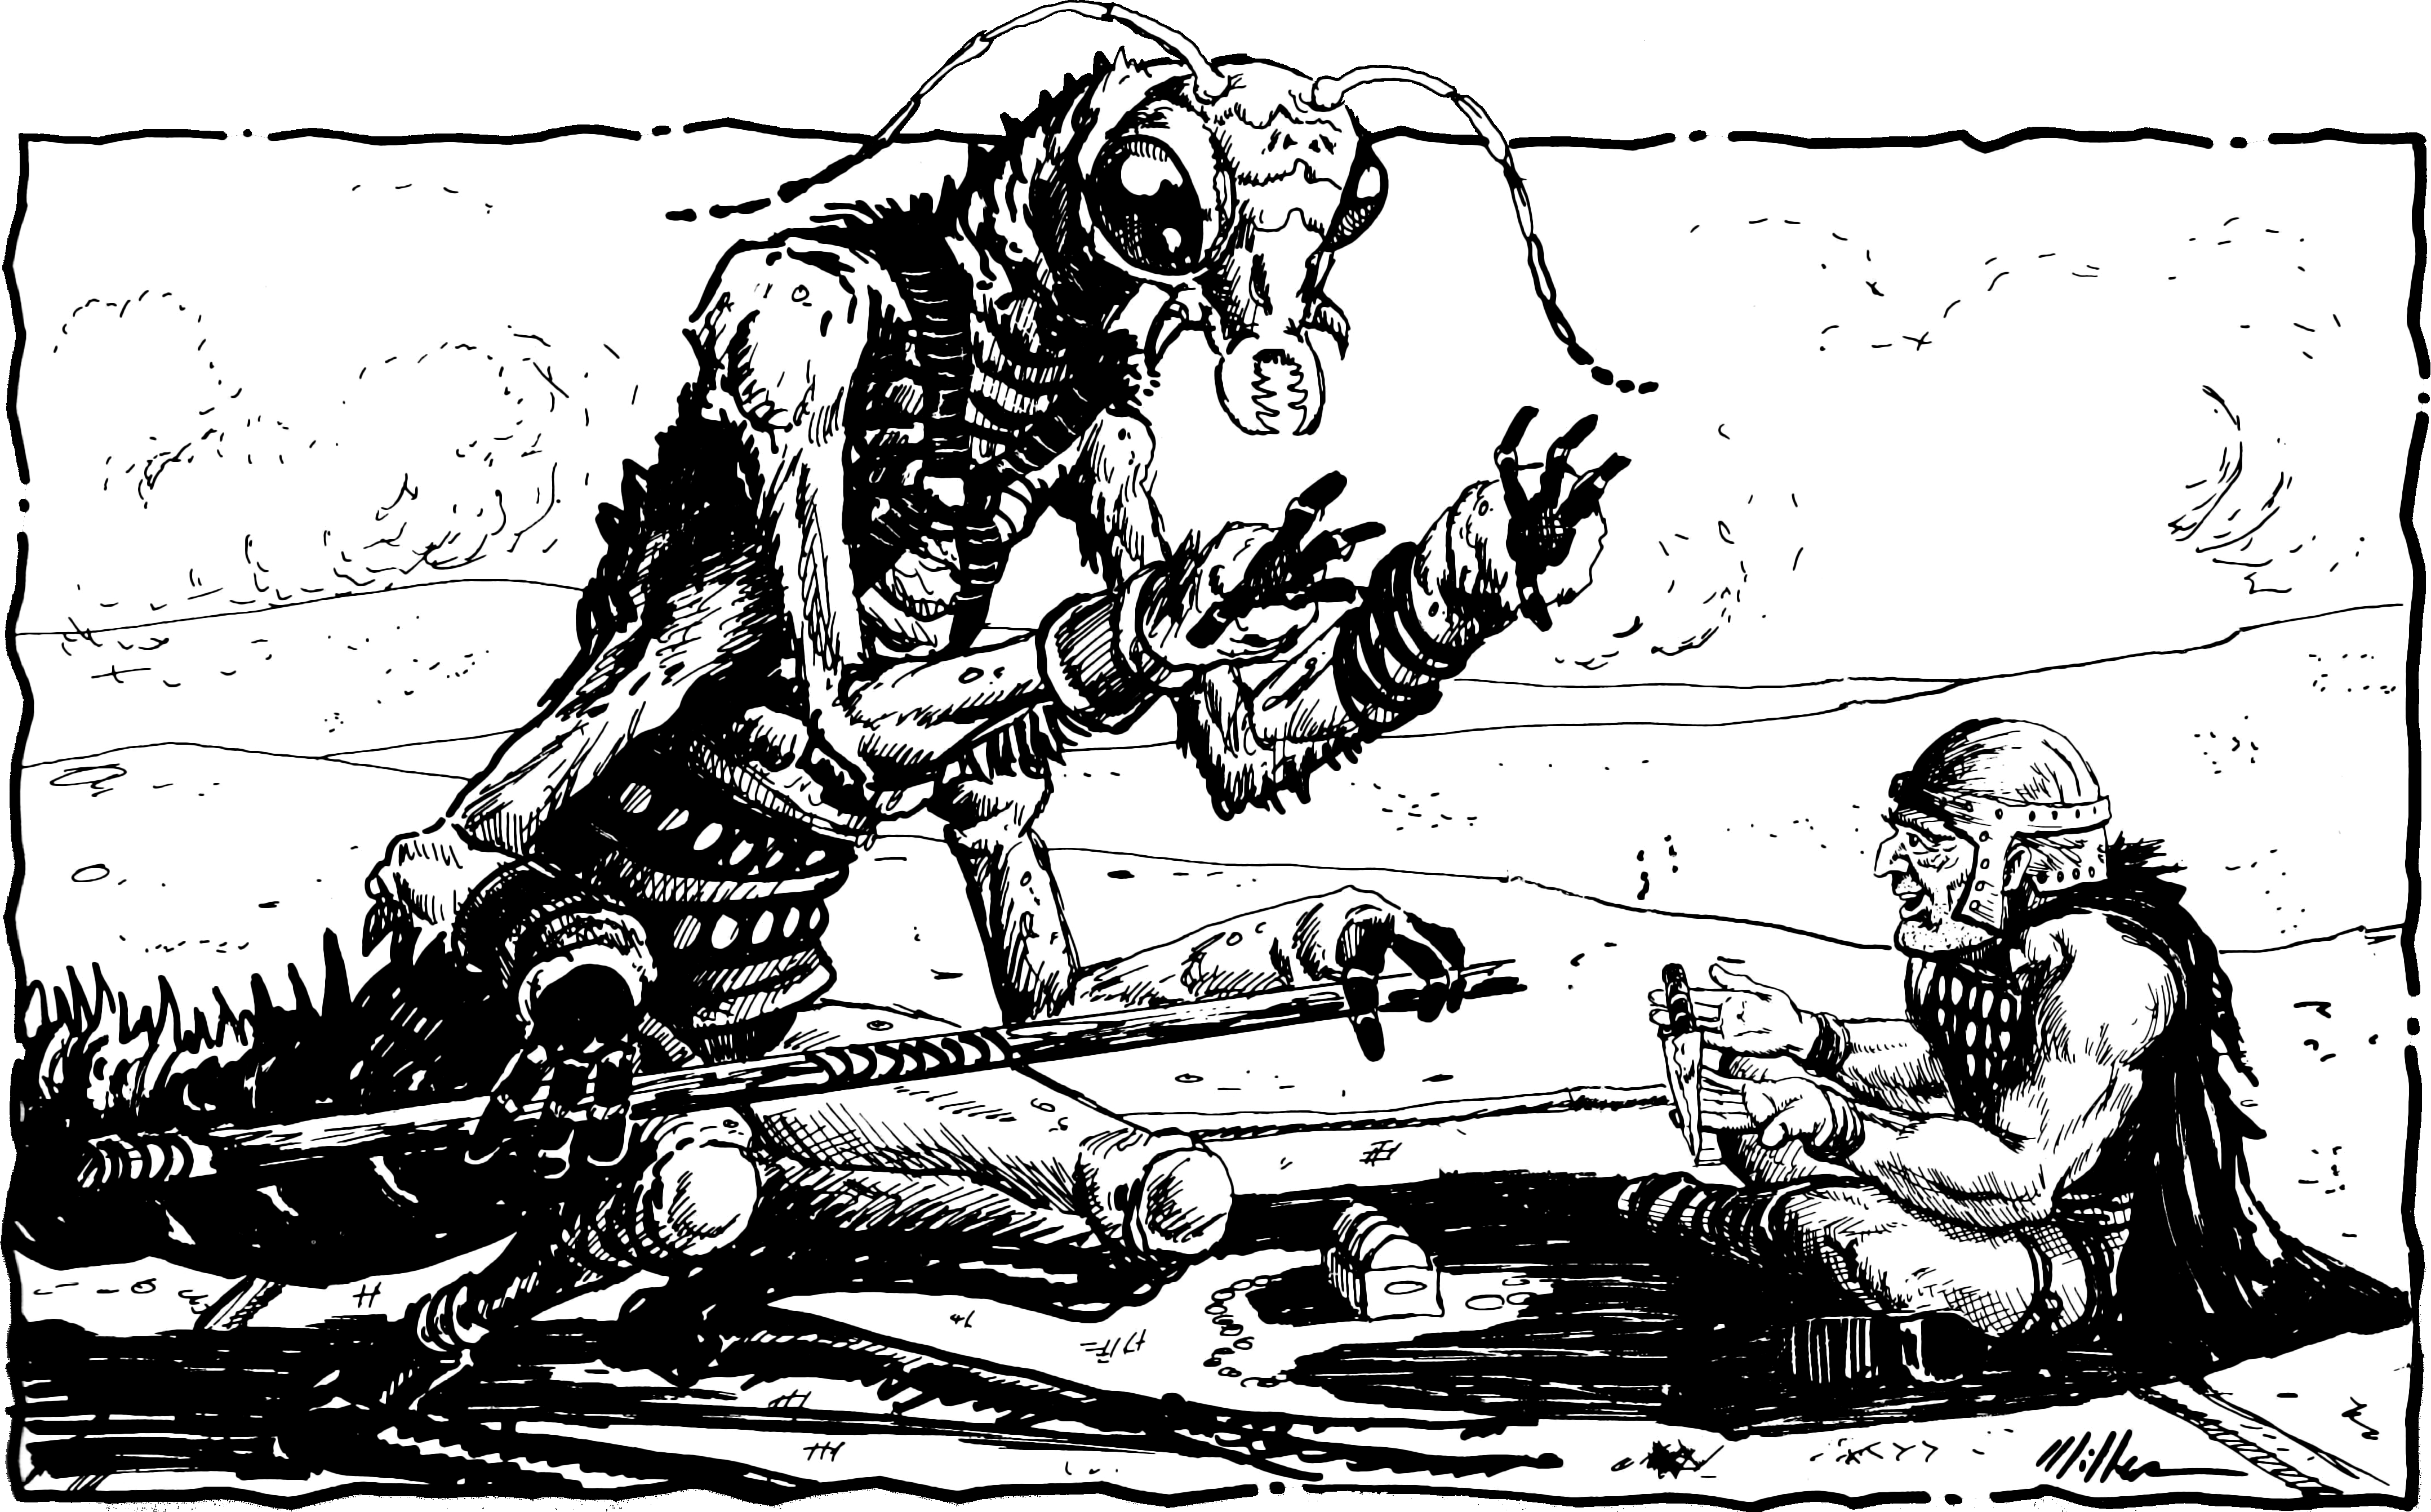
\includegraphics[width=\textwidth]{images/merchant-3.png}
\par\textit{\small\textcopyright Wizards of the Coast, 2020.}
\end{figure*}
\subsection{Documents}
This class of items has a symbolic function, conveying authority or permission. No price is listed for these items, because their value is not inherent.

\textbf{Letter of Marque}: This letter bears the personal mark of the sorcerer‐king, and bestows limited secular authority on the bearer, as if the bearer were a templar. The bearer of a letter of marque gains the authority to contest the actions of templars, using the bearer’s \skill{Diplomacy} check. If the bearer is already a templar, then having the letter as additional authority grants the templar a +4 circumstance check towards authority contest checks. The letter of marque does not grant the authority to Intrude, Requisition, Accuse or Judge, but does grant power to contest such actions by templars. A letter of marque is limited by time. After a specified period (usually one year, and never longer than seven years) the letter loses its effectiveness. A sorcerer‐king can also declare the letter invalid. Forging or fraudulently using a letter of marque is an unpardonable offense that brings a death sentence. Obviously, only the templars and other servants of the sorcerer‐king that issued the letter of marque will honor its terms. A person who is caught with a king’s letter of marque within another sorcerer‐king’s territory will have some explaining to do.

\textbf{Letter of Reprisal}: Like a letter of marque, this letter bears the personal mark of the sorcerer‐king, and bestows limited secular authority on the bearer, as if the bearer were a templar. Unlike a letter of marque, a letter of reprisal has a limited scope to carrying out a specific mission, usually a reprisal or retaliation against a specific group of the King’s enemies, for example, killing or capturing a specific enemy officer, capturing a particular enemy fortress or silt vessel, defiling a stretch of key farmland, or annihilating or enslaving a designated village. Depending on the bearer’s \skill{Diplomacy} ranks, she can Requisition, Intrude, Accuse, Judge, but only if she can show that her request relates to fulfilling her assigned mission. She can attempt to contest the actions of other templars, but takes a $-4$ circumstance penalty on such attempts, since the opposing templars can argue (even if it is not true) that she is acting outside of the scope of the assigned reprisal mission. The $-4$ penalty also applies if templars contest any of her Requisition, Intrude, Accuse, or Judge actions.
\subsectionA{Food, Drink, and Lodging}
Many Athasian travelers are lodged by merchant houses, elemental temples, psionic academies, or family. Adventurers, however, pay for hospitality.

\Table{Food, Drink, and Lodging}{XRR}{
\tableheader Item & \tableheader Cost & \tableheader Weight\\
\TableSubheader{Broy} &&\\
~ Keg (4 liters) & 2 cp & 5 kg\\
~ Mug & 4 bits & \onehalf kg\\
\TableSubheader{Inn stay (per day)} &&\\
~ Good & 2 sp & \\
~ Common & 5 cp & \\
~ Poor & 2 cp & \\
\TableSubheader{Meals (per day)} &&\\
~ Good & 5 bits & \\
~ Common & 3 bits & \\
~ Poor & 1 bit & \\
\TableSubheader{Water} &&\\
~ Keg (4 liters) & 2 bits & 5 kg\\
~ Mug & 1 bd & \onehalf kg\\
}

\textbf{Broy:} Broy is made from fermented kank nectar. Spiced broy and watered-down broy are also available. When served plain, it is potent and foul tasting. However, broy can be served warm and spiced with a pungent herb that disguises its sourness, as well as enhancing its enrapturing powers.

\textbf{Inn:} Poor accommodations at an inn amount to a place on the floor near the hearth. Common accommodations consist of a place on a raised, heated floor, the use of a blanket and a pillow. Good accommodations consist of a small, private room with one bed, some amenities, and a covered chamber pot in the corner.

\textbf{Meals:} Poor meals might be composed of bread, baked turnips, onions, and water. Common meals might consist of bread, chicken stew, carrots, and watered-down ale or wine. Good meals might be composed of bread and pastries, beef, peas, and ale or wine.
\subsectionA{Mounts and Related Gear}

\Table{Mounts and Related Gear}{XRR}{
\tableheader Goods or Services & \tableheader Cost & \tableheader Weight \\
\TableSubheader{Barding} &&\\
~ Medium creature & $\times$2 & $\times$1 \\
~ Large creature & $\times$4 & $\times$2 \\
Bit and bridle & 2 cp & \onehalf kg \\
Feed (per day) & 1 bit & 5 kg \\
\TableSubheader{Mounts} &&\\
~ \TableSubheader{Birds} &&\\
~ Erdland & 25 cp &\\
~ Erdlu & 10 cp &\\
~ \TableSubheader{Reptiles} &&\\
~ Crodlu, riding & 200 cp & \\
~ Crodlu, warmount & 400 cp & \\
~ Inix & 100 cp & \\
~ Mekillot & 200 cp & \\
~ \TableSubheader{Insects} &&\\
~ Kank, herding & 50 cp &\\
~ Kank, riding & 125 cp &\\
~ Kank, warmount & 250 cp &\\
\TableSubheader{Saddle} &&\\
~ Military & 20 cp & 15 kg \\
~ Pack & 5 cp & 7.5 kg \\
~ Riding & 10 cp & 12.5 kg \\
\TableSubheader{Saddle, Exotic} &&\\
~ Military & 60 cp & 20 kg \\
~ Pack & 15 cp & 10 kg \\
~ Riding & 30 cp & 15 kg \\
Saddlebags & 4 cp & 4 kg \\
Stabling (per day) & 5 bits &\\
}

\textbf{Barding, Medium Creature and Large Creature:} Barding is a type of armor that covers the head, neck, chest, body, and possibly legs of a horse or other mount. Barding made of medium or heavy armor provides better protection than light barding, but at the expense of speed. Barding can be made of any of the armor types found on \tabref{Armor and Shields}.

Armor for a horse (a Large nonhumanoid creature) costs four times as much as armor for a human (a Medium humanoid creature) and also weighs twice as much as the armor found on \tabref{Armor and Shields} (see Armor for Unusual Creatures). If the barding is for a pony or other Medium mount, the cost is only double, and the weight is the same as for Medium armor worn by a humanoid. Medium or heavy barding slows a mount that wears it, as shown on the table below.

Flying mounts can't fly in medium or heavy barding.

Removing and fitting barding takes five times as long as the figures given on \tabref{Donning Armor}. A barded animal cannot be used to carry any load other than the rider and normal saddlebags.

\Table{Barding}{XCCC}{
 & \multicolumn{3}{c}{\tableheader Base Speed}\\
\cmidrule[0.5pt]{2-4}
\tableheader Barding & \tableheader (12 m) & \tableheader (15 m) & \tableheader (18 m)\\
Medium & 9 m & 10.5 m & 12 m\\
Heavy & 9 m\footnotemark[1] & 10.5 m\footnotemark[1] & 12 m\footnotemark[1]\\

\TableNote{4}{1 A mount wearing heavy armor moves at only triple its normal speed when running instead of quadruple.}\\
}

\textbf{Crodlu:} A crodlu is a large bipedal lizard mount, resembling a scaled ostrich. A crodlu is appropriate as a mount for a Medium humanoid creature. Crodlu are hard to control in battle, while war crodlu can be ridden into battle easily. Crodlu benefit from stabling, can wear barding, and require feed like normal mounts.

\textbf{Erdland:} These creatures are large, flightless birds used as mounts or to pull caravans. They weigh around 2 tons and can stand up to 4.5 meters tall. An erdland is appropriate as a mount for a Medium humanoid creature. Erdlands can be ridden into battle easily. Erdlands benefit from stabling, can wear barding, and require feed like normal mounts.

\textbf{Erdlu:} Erdlus are a smaller variety of erdland, mostly used as herd beasts. They stand 2.1 meters tall and weigh around 100 kg. An erdlu is appropriate as a mount for a Medium humanoid creature. Erdlus are hard to control in battle. Erdlus benefit from stabling, can wear barding, and require feed like normal mounts.

\textbf{Feed:} Crodlus, erdlands, erdlus, inixes require feeding. Mekillots require eight times more than normal mounts.

\textbf{Inix:} The inix is a large, 5.5-meter long reptile commonly used for riding and as a beast of burden. An inix is appropriate as a mount for a Medium or Large humanoid creature. Inixes can be ridden into battle easily. Inixes benefit from stabling, can wear custom barding (specially constructed, adding an additional 50\% to the price), and require feed like normal mounts.

\textbf{Kank:} A kank is a large, 2.4-meter long insect, commonly used as a personal mount. These insects cannot be used as food, for their meat smells atrocious, but they produce highly nutritious globules of honey. A kank is appropriate as a mount for a Medium humanoid creature. Kanks are hard to control in battle. Kanks benefit from stabling, cannot wear barding, and do not require feeding.

\textbf{Mekillot:} A mekillot is a huge, 3,000-kg. lizard, used for hauling large cargo or serving as transportation for troops. These beasts are hard to control in combat and usually require a psionic handler. Mekillots benefit from stabling, can wear barding, and require feed eight times more than a normal mount.

\textbf{Saddle, Exotic:} An exotic saddle is like a normal saddle of the same sort except that it is designed for an unusual mount. Exotic saddles come in military, pack, and riding styles.

\textbf{Saddle, Military:} A military saddle braces the rider, providing advantage on \skill{Ride} checks related to staying in the saddle. If you're knocked unconscious while in a military saddle, you have a 75\% chance to stay in the saddle (compared to 50\% for a riding saddle).

\textbf{Saddle, Pack:} A pack saddle holds gear and supplies, but not a rider. It holds as much gear as the mount can carry.

\textbf{Saddle, Riding:} The standard riding saddle supports a rider.

\clearpage
\begin{figure}[t!]
\centering
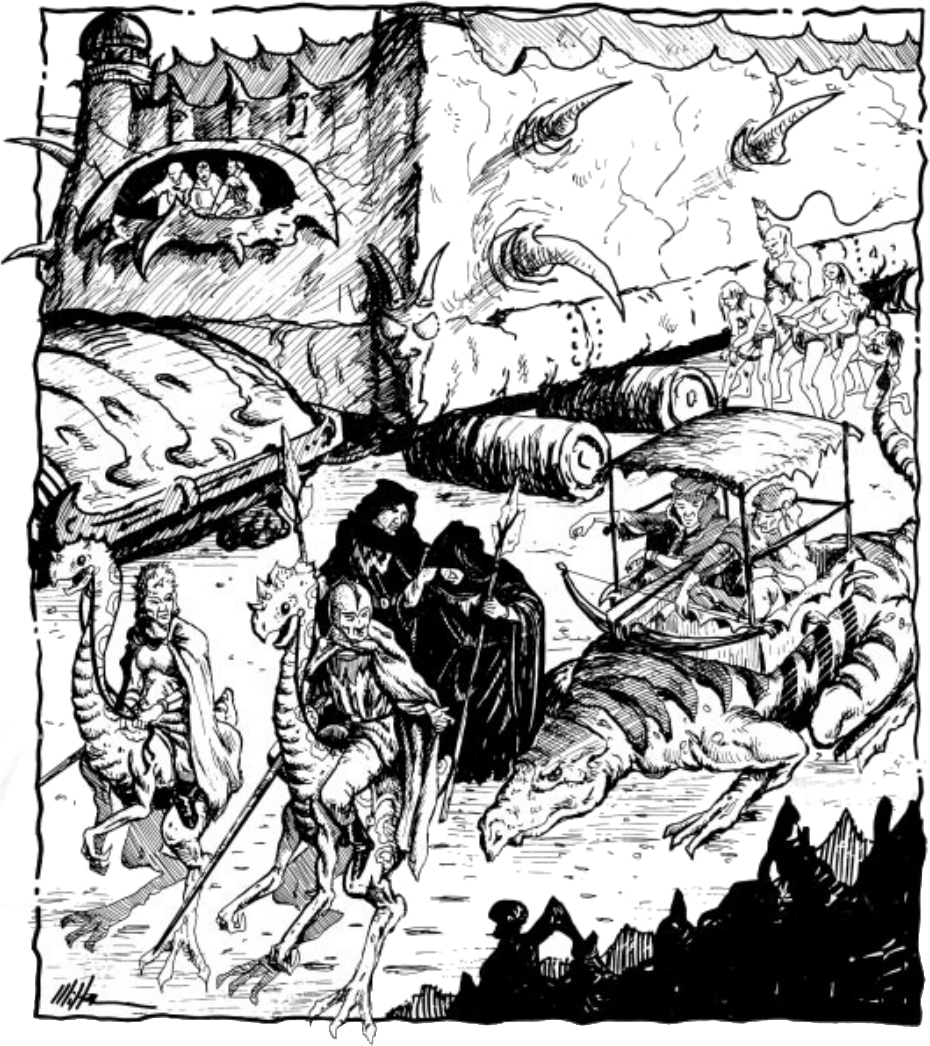
\includegraphics[width=\columnwidth]{images/caravan-3.png}
\par\textit{\small\textcopyright Wizards of the Coast, 2020.}
\end{figure}
\subsection{Transport}
Sometimes it is too hard or too dangerous to ride a kank---you'll need some other form of transportation. Some vehicles, such as the chariot and howdah, are moved by muscle power. The \skill{Handle Animal} skill is used only if that power comes from a team of draft animals. When the team consists of creatures with Intelligence scores of 3 or higher, the operative skill is \skill{Diplomacy}. When they are slaves or forced labor, the operative skill is \skill{Intimidate}.

\Table{Transport}{Xr{2cm}}{
\tableheader Transport & \tableheader Cost\\
Chariot, two-person, transport & 50 cp \\
Chariot, two-person, war & 125 cp \\
Chariot, four-person, war & 250 cp \\
Howdah, inix & 10 cp \\
Howdah, inix, war & 100 cp \\
Howdah, mekillot & 20 cp \\
Howdah, mekillot, war & 500 cp \\
Wagon, open, 500 kg capacity & 20 cp \\
Wagon, open, 1,250 kg capacity & 35 cp \\
Wagon, open, 2,500 kg capacity & 50 cp \\
Wagon, open, 5,000 kg capacity & 100 cp \\
Wagon, enclosed, 500 kg capacity & 40 cp \\
Wagon, enclosed, 1,250 kg capacity & 70 cp \\
Wagon, enclosed, 2,500 kg capacity & 100 cp \\
Wagon, enclosed, 5,000 kg capacity & 200 cp \\
Wagon, armored caravan & 1,000 cp \\
}

\textbf{Chariot}: A chariot is a two‐wheeled vehicle used for transportation, racing, war and processions. Transport chariots are very small and simple, requiring only a single animal to draw it. A war chariot built for two riders is slightly larger, but significantly better constructed. Generally one person will drive the chariot while the other uses a bow or other ranged weapon. A war chariot built for four is much larger than the other two kinds of chariots and requires at least two mounts to drive it. A war chariot offers cover to its occupants.

\textbf{Howdah}: A howdah is an enclosure mounted on a riding animal containing space for one or more persons. Howdahs can be fitted on inix or mekillots, and provide shade and cover from the elements. An inix howdah usually has room for only one person, though the war howdah, built much stronger, can hold four. A mekillot howdah can hold one or two persons, but a war howdah is much bigger, consisting of two levels and holding up to sixteen warriors.

\textbf{Wagon}: Wagons are an essential part of Athasian economy, as they facilitate the caravans that make life in the wastes possible. Open wagons are basic, open–topped wagons that can carry a certain amount of cargo. As Athasian wagons are built using little or no metal, there’s a limit to how much cargo they can carry. Open wagons generally require two beasts to draw them, but sometimes a single erdland will work.

\textit{Enclosed wagons}: They are more commonly used to transport people or fragile cargo that would otherwise be damaged by exposure to the elements.

\textit{Armored wagons}: They are primarily used by caravans traveling through areas plagued by dangerous monsters or raiders. It is an enclosed wagon with agafari wood used to strengthen the wagon throughout. There are also mount points for fixed crossbows on each side of that wagon that can swivel 180 degrees. Anyone using the crossbows or firing out of the rear of the wagon (when it is open) receives cover. Armored wagons require at least four smaller mounts to draw it, two inixes or one mekillot.

\subsectionA{Services}

\Table{Services}{lR}{
\tableheader Services & \tableheader Cost\\
Messenger         & 1 bit/km\\
Road or gate toll & 1 bit\\

\multicolumn{2}{l}{\TableSubheader{Hirelings, Military}}\\
Archer              & 1 bit/day  \\
Cavalry, heavy      & 3 bits/day \\
Cavalry, light      & 1 bit/day  \\
Crossbowman         & 5 bd/day   \\
Engineer            & 5 cp/day   \\
Infantry, heavy     & 5 bd/day   \\
Infantry, light     & 2 bd/day   \\
Infantry, irregular & 1 bd/day   \\

\multicolumn{2}{l}{\TableSubheader{Hirelings, Civilian}}\\
Draqoman                        & Level in cp/day \\
Craftsman\footnotemark[1]       & 1 bit/day      \\
Professional\footnotemark[2]    & 5 bd/day       \\
Specialist\footnotemark[3]      & 3 bits/day     \\
Spellcaster                     & 5 bits/day     \\
Unskilled labor\footnotemark[4] & 2 bd/day       \\


\multicolumn{2}{l}{\TableSubheader{Manifesting}}\\
Power, 1st--level & Manifester level $\times$ 10 cp\footnotemark[5]\\
Power, 2nd--level & Manifester level $\times$ 20 cp\footnotemark[5]\\
Power, 3rd--level & Manifester level $\times$ 30 cp\footnotemark[5]\\
Power, 4th--level & Manifester level $\times$ 40 cp\footnotemark[5]\\
Power, 5th--level & Manifester level $\times$ 50 cp\footnotemark[5]\\
Power, 6th--level & Manifester level $\times$ 60 cp\footnotemark[5]\\
Power, 7th--level & Manifester level $\times$ 70 cp\footnotemark[5]\\
Power, 8th--level & Manifester level $\times$ 80 cp\footnotemark[5]\\
Power, 9th--level & Manifester level $\times$ 90 cp\footnotemark[5]\\

\multicolumn{2}{l}{\TableSubheader{Spellcasting}}\\
Spell,   0--level & Caster level $\times$  5 sp\footnotemark[5]\footnotemark[6]\\
Spell, 1st--level & Caster level $\times$ 10 sp\footnotemark[5]\footnotemark[6]\\
Spell, 2nd--level & Caster level $\times$ 20 sp\footnotemark[5]\footnotemark[6]\\
Spell, 3rd--level & Caster level $\times$ 30 sp\footnotemark[5]\footnotemark[6]\\
Spell, 4th--level & Caster level $\times$ 40 sp\footnotemark[5]\footnotemark[6]\\
Spell, 5th--level & Caster level $\times$ 50 sp\footnotemark[5]\footnotemark[6]\\
Spell, 6th--level & Caster level $\times$ 60 sp\footnotemark[5]\footnotemark[6]\\
Spell, 7th--level & Caster level $\times$ 70 sp\footnotemark[5]\footnotemark[6]\\
Spell, 8th--level & Caster level $\times$ 80 sp\footnotemark[5]\footnotemark[6]\\
Spell, 9th--level & Caster level $\times$ 90 sp\footnotemark[5]\footnotemark[6]\\

\TableNote{2}{1 Any \skill{Craft} skill available.}\\
\TableNote{2}{2 Any \skill{Profession} skill available.}\\
\TableNote{2}{3 Any skill, other than Craft and Profession.}\\
\TableNote{2}{4 Jobs that do not require associated skills.}\\
\TableNote{2}{5 See its description for additional costs. If the additional costs put the total cost above 3,000 cp, that service is not generally available.}\\
\TableNote{2}{6 Spellcasting is considered high treason and spellcasters are not comfortable offering their services.}\\
}

Sometimes the best solution for a problem is to hire someone else to take care of it. Spellcasting, unless divine, is rarely, if ever, for sale on Athas. However, the manifesting of psionic powers for cash is much more common.

\textbf{Archer:} A 2nd-level fighter specialized in longbows, weilding a composite longbow (Str +2), and wearing studded leather and a buckler.

\textbf{Cavalry, Heavy:} A 2nd-level fighter wearing scale mail, and wielding a lance two-handed. They mount a heavy crodlu wearing a scale mail, as well.

\textbf{Cavalry, Light:} A 1st-level fighter wearing a studded leather and a wooden shield, and wielding a lance. They mount a light crodlu with no armor.

\textbf{Craftsman:} Usually a 2nd-level settler, but they can be of any class. This pays for any \skill{Craft} check of DC 20 or lower. Higher DC checks double the price for each 5 points of difference. 

\textbf{Crossbowman:} A 1st-level fighter specialized in crossbows, weilding a composite heavy crossbow (Str +4), and wearing studded scale mail and a tower shield.

\textbf{Draqoman:} A bard of 6th or higher level with at least one contact (see Alternative Class Features). Their wages depends on the bard's level and are the default price for skill contacts. If the draqoman has different types of contact, then they might double the price.

\textbf{Engineer:} A 5th-level fighter with 8 ranks of \skill{Knowledge} (warcraft) and a martial prowess that depend on this skill. They are equipped with \emph{breastplate +1} and a \emph{tower shield +1}. Although a military engineer has combat capabilities, their function is to oversee construction of siege engines and of static defenses.

\textbf{Infantry, Heavy:} A 2nd-level fighter, wearing a half-plate and tower shield, wielding a one-handed weapon. 

\textbf{Infantry, Light:} A 1st-level fighter, specialized either in spear and shields, or longswords. Light infantry usually wears studded leather, but caravan's infantry wear caravan armor.

\textbf{Infantry, Irregular:} A 2nd-level barbarian or gladiator. Their specialization is atypical, and they typically use gladiator armor or shell armor.

\textbf{Messenger:} This entry includes mounted messengers and runners. Those willing to carry a message to a place they were going anyway may ask for only half the indicated amount.

\textbf{Power:} The indicated amount is how much it costs to get a manifester to manifest a power for you. This cost assumes that you can go to the manifester and have the power manifested at his or her convenience. If you want to bring the manifester somewhere to manifest a power you need to negotiate with the manifester, otherwise the default answer is no.

The cost given is for a power with no XP cost. If the power has an XP cost, add 5 cp per XP lost.

Furthermore, if a power has dangerous consequences, the manifester will certainly require proof that you can and will pay for dealing with any such consequences (that is, assuming that the manifester even agrees to manifest such a power, which isn't certain). In the case of powers that transport the manifester and characters over a distance, you will likely have to pay for two manifestations of the power, even if you aren't returning with the manifester.

In addition, not every town or village has a manifester of sufficient level to manifest any power. In general, you must travel to a small town (or larger settlement) to be reasonably assured of finding a manifester capable of manifesting 1st--level powers, a large town for 2nd--level powers, a small city for 3rd-- or 4th--level powers, a large city for 5th-- or 6th--level powers, and a metropolis for 7th-- or 8th--level powers. Even a metropolis isn't guaranteed to have a local manifester able to cast 9th--level powers.

\textbf{Professional:} Usually a 2nd-level settler, but they can be of any class. This pays for any \skill{Profession} check of DC 20 or lower. Higher DC checks double the price for each 5 points of difference.

\textbf{Road or Gate Toll:} A toll is sometimes charged to cross a well-trodden, well-kept, and well-guarded road to pay for patrols on it and for its upkeep. Occasionally, a large walled city charges a toll to enter or exit (or sometimes just to enter).

\textbf{Specialist:} A 2nd-level NPC with \feat{Skill Focus} on the corresponding skill speciality, who can deliver a skill check of DC 20. Scouts are usually hired for \skill{Knowledge} (geography), \skill{Spot}, or \skill{Survival}. Thieves for \skill{Disable Device}, \skill{Forgery}, \skill{Open Lock}, \skill{Search}, or \skill{Sleight of Hand}. Bards for \skill{Appraise}, \skill{Diplomacy}, or \skill{Perform}. Wizards for \skill{Decipher Script}, any \skill{Knowledge}, or \skill{Spellcraft}. These are guidelines, but the wages are the same for any class.

\textbf{Spell:} The indicated amount is how much it costs to get a spellcaster to cast a spell for you. This cost assumes that you can go to the spellcaster and have the spell cast at his or her convenience (generally at least 24 hours later, so that the spellcaster has time to prepare the spell in question). If you want to bring the spellcaster somewhere to cast a spell you need to negotiate with him or her, and the default answer is no.

The cost given is for a spell with no cost for a material component or focus component and no XP cost. If the spell includes a material component, add the cost of that component to the cost of the spell.

If the spell has a focus component (other than a divine focus), add 1/10 the cost of that focus to the cost of the spell. If the spell has an XP cost, add 5 cp per XP lost.

Furthermore, if a spell has dangerous consequences, the spellcaster will certainly require proof that you can and will pay for dealing with any such consequences (that is, assuming that the spellcaster even agrees to cast such a spell, which isn't certain). In the case of spells that transport the caster and characters over a distance, you will likely have to pay for two castings of the spell, even if you aren't returning with the caster.

In addition, not every town or village has a spellcaster of sufficient level to cast any spell. In general, you must travel to a small town (or larger settlement) to be reasonably assured of finding a spellcaster capable of casting 1st--level spells, a large town for 2nd--level spells, a small city for 3rd-- or 4th--level spells, a large city for 5th-- or 6th--level spells, and a metropolis for 7th-- or 8th--level spells. Even a metropolis isn't guaranteed to have a local spellcaster able to cast 9th--level spells.

\textbf{Spellcaster:} A 3rd-level cleric or wizard. These wages do not pay for expensive material components, which must be given by the employer.

\textbf{Unskilled Labor:} Any job that a freeman might do that does not require a skill check.

